%%%%%%%%%%%%%%%%%%%%%%%%%%%%%%%%%%%%%%%%%%%%%%%%%%%%%%%%%%%%%%%%%%%%%%%%%%%%%%%%
%2345678901234567890123456789012345678901234567890123456789012345678901234567890
%        1         2         3         4         5         6         7         8

\documentclass[letterpaper, 10 pt, conference]{ieeeconf}  % Comment this line out if you need a4paper

%\documentclass[a4paper, 10pt, conference]{ieeeconf}      % Use this line for a4 paper

\IEEEoverridecommandlockouts                              % This command is only needed if
                                                          % you want to use the \thanks command

\overrideIEEEmargins                                      % Needed to meet printer requirements.

% ---- packages ---------------------------------------------------------------
\usepackage{amsmath}
\usepackage{amssymb}
\usepackage{graphicx}
\usepackage{booktabs}
\usepackage{siunitx}
\usepackage{cite}
\usepackage{url}

% ---- hyphenation hints -------------------------------------------------------
\hyphenation{HERACLES ngspice compute-in-memory}

% ---- macros -----------------------------------------------------------------
\newcommand{\VT}{V_{\mathrm{T}}}
\newcommand{\NMED}{\mathrm{NMED}}
\newcommand{\sigDD}{\sigma_{\mathrm{D2D}}}
\newcommand{\sigNMED}{\sigma_{\mathrm{NMED}}}
\newcommand{\VDD}{V_{\mathrm{DD}}}

% =============================================================================
\title{\LARGE \bf
FeFET-Based Approximate Arithmetic for Energy-Efficient
Compute-in-Memory%
}

\author{Nakshat Pandey$^{1}$, Sushant Kumar$^{1}$, Santhosh Sivasubramani$^{2}$%
\thanks{$^{1}$N.~Pandey and S.~Kumar are with the Department of Electrical
        Engineering, IIT Delhi, New Delhi 110016, India
        {\tt\small \{e1221436, ee1222045\}@iitd.ac.in}}%
\thanks{$^{2}$S.~Sivasubramani is with the Centre for Sensors, Instrumentation
        and Cyber Physical Systems Engineering (SeNSE), IIT Delhi, New Delhi
        110016, India
        {\tt\small ssivasub@iitd.ac.in}}%
}


\begin{document}

\maketitle
\thispagestyle{empty}
\pagestyle{empty}


%%%%%%%%%%%%%%%%%%%%%%%%%%%%%%%%%%%%%%%%%%%%%%%%%%%%%%%%%%%%%%%%%%%%%%%%%%%%%%%%
\begin{abstract}

Ferroelectric FET (FeFET) devices offer two stable threshold-voltage states,
making them natural candidates for non-volatile compute-in-memory (CiM)
applications. In this work, we investigate the synergy between FeFET
variability and approximate arithmetic: device-to-device $\VT$ variation is a
key reliability concern in CiM, and approximate circuits---which accept bounded
output errors by design---may be inherently more amenable to such variation
than exact counterparts. We implement and characterize four approximate
circuits---LOA-8, HEAA-8, AMA5-8, and BAM~$4\times4$---in both CMOS 45\,nm
and FeFET technologies using ngspice~45.2 with the HERACLES compact model.
CMOS 45\,nm results confirm that approximate circuits achieve 35--51\% lower
propagation delay and up to 68\% power reduction versus exact counterparts at
$\NMED < 0.008$. FeFET BAM~$4\times4$ achieves 92.3\,ps delay and 10.9\,fJ
PDP, a 70\% PDP reduction over the CMOS baseline. Monte Carlo variability
analysis across $\sigDD = 20$--$100$\,mV confirms zero NMED variation
($\sigNMED = 0.000$) in all circuits, confirming that approximate-circuit
accuracy is robust to FeFET $\VT$ variability across the practical range of
device-to-device variation.

\end{abstract}

\smallskip\noindent\textbf{Keywords}---FeFET; approximate computing;
compute-in-memory; approximate adder; approximate multiplier; variability
tolerance.


%%%%%%%%%%%%%%%%%%%%%%%%%%%%%%%%%%%%%%%%%%%%%%%%%%%%%%%%%%%%%%%%%%%%%%%%%%%%%%%%
\section{Introduction}

The scaling limits of CMOS have spurred interest in emerging non-volatile
memory (NVM) technologies for in-memory computing. Among these, ferroelectric
FETs (FeFETs) are particularly attractive: their polarization-controlled
threshold voltage enables non-destructive, multi-level cell reading directly
within the logic gate, eliminating the costly data-movement bottleneck of
von~Neumann architectures~\cite{jerry2017fefet}.

At the same time, many real-world applications---image processing, machine
learning inference, and signal processing---can tolerate bounded computational
errors. Approximate computing deliberately exploits this tolerance to trade
accuracy for energy efficiency and speed. Prior work has demonstrated that
approximate adders such as LOA~\cite{gupta2013loa}, HEAA~\cite{ye2013heaa},
and AMA5~\cite{almurib2018ama5}, and approximate multipliers such as
BAM~\cite{momeni2015bam}, achieve 30--50\% power and delay savings with small
quality loss.

This paper explores the intersection of these two paradigms. We hypothesize
that approximate circuits are robust to FeFET $\VT$ variability by virtue of
their pre-accepted error tolerance. Since approximate circuits already accept
bounded output errors, the additional error introduced by $\VT$ mismatch
($\sigDD \sim 40$\,mV) may fall within the pre-defined error tolerance,
enabling robust CiM operation without added error-correction overhead.

Our contributions are: (1)~ngspice-based characterization of four approximate
circuits in CMOS 45\,nm and FeFET technologies; (2)~quantification of CMOS
timing, power, and error metrics; (3)~FeFET circuit performance benchmarking
using the HERACLES compact model~\cite{heracles2022}; and (4)~Monte Carlo and
sigma-sweep variability analysis confirming zero NMED degradation
($\sigNMED = 0$) across $\sigDD = 20$--$100$\,mV.


%%%%%%%%%%%%%%%%%%%%%%%%%%%%%%%%%%%%%%%%%%%%%%%%%%%%%%%%%%%%%%%%%%%%%%%%%%%%%%%%
\section{Circuit Design and FeFET Encoding}

\subsection{FeFET Encoding Scheme}

FeFETs are modeled using the HERACLES compact model~\cite{heracles2022}, which
extends BSIM4 with a ferroelectric-capacitor polarization sub-circuit. Two
stable polarization states correspond to $\VT^{\mathrm{low}} \approx 0.35$\,V
(logic~`1' stored) and $\VT^{\mathrm{high}} \approx 1.5$\,V (logic~`0'
stored). The device reads non-destructively during regular circuit operation,
making it suitable for CiM.

In our implementation, FeFET devices replace nMOS transistors in the pull-down
networks of approximate cells. The approximate lower-bit cells (bits~0 to
$k{-}1$) use pseudo-nMOS FeFET AND/OR gates with a PMOS keeper. The upper
exact bits retain standard CMOS full-adder topology (mirror adder) with FeFETs
in the carry pull-down path.

\subsection{Approximate Adder Designs}

Three 8-bit approximate adders are implemented with $k = 4$ approximate lower
bits and $k = 4$ exact upper bits:

\textbf{LOA-8} (Lower-part OR Adder)~\cite{gupta2013loa}: The lower $k$ bits
replace full adders with simple OR gates, eliminating carry logic in the
approximate region. This reduces transistor count from 224 (RCA-8) to~142
(37\% reduction) and delay from 181.4\,ps to 107.8\,ps.

\textbf{HEAA-8} (Hybrid Error-tolerant Adder Architecture)~\cite{ye2013heaa}:
Uses an XOR-based approximate cell for the lower bits. Achieves the lowest
$\NMED$ (0.0034) among the three adders with 156~transistors.

\textbf{AMA5-8} (Approximate Mirror Adder~5)~\cite{almurib2018ama5}: Employs
a ratioed-logic approximate full adder. Most aggressive design: only
112~transistors (50\% reduction vs.\ RCA-8), but highest $\NMED$ (0.0078) and
error rate (93.8\%).

\subsection{Approximate Multiplier Design}

\textbf{BAM~$4\times4$} (Broken Array Multiplier, $v = 2$)~\cite{momeni2015bam}:
A 4-bit$\,\times\,$4-bit multiplier where the lower 2~columns of partial
products are truncated. Reduces transistor count from 296 to~224 with
$\NMED = 0.0049$. FeFET implementation shows significant PDP improvement
(10.9\,fJ vs.\ 36.7\,fJ CMOS) due to lower switching currents in FeFET
pull-down paths.


%%%%%%%%%%%%%%%%%%%%%%%%%%%%%%%%%%%%%%%%%%%%%%%%%%%%%%%%%%%%%%%%%%%%%%%%%%%%%%%%
\section{Simulation Methodology}

All simulations use ngspice~45.2 in Docker with the OSDI interface for
Verilog-A models. The CMOS 45\,nm baseline uses the PTM~45\,nm HP model
(\texttt{ptm45\_hp.pm}) at $\VDD = 1.0$\,V. FeFET circuits use HERACLES
(OSDI) with $\VT^{\mathrm{low}} = 0.35$\,V, $\VT^{\mathrm{high}} = 1.5$\,V,
$\sigDD = 40$\,mV, $\sigma_{\mathrm{C2C}} = 20$\,mV.

\textbf{Timing characterization:} Each circuit is driven with the worst-case
input vector that exercises the longest carry-ripple path. Propagation delay
($t_{\mathrm{pd}}$) is measured as the 50\% crossing time from the triggering
input transition to the output response using the ngspice
\texttt{.measure}~TRIG/TARG directive.

\textbf{Power characterization:} Average power is measured during an
exhaustive all-inputs-switching pattern at 1\,GHz clock frequency.
Power-delay product $\mathrm{PDP} = t_{\mathrm{pd}} \times \bar{P}_{\mathrm{avg}}$.

\textbf{Error metrics:} NMED, MRED, ER, and WCE are computed from exhaustive
input truth tables ($2^{8}$ for 8-bit adders; $2^{4}\times2^{4}$ for the
$4\times4$ multiplier) using Python analysis scripts.

\textbf{Monte Carlo variability:} Per-circuit iteration counts of 200~(LOA-8),
50~(HEAA-8), 200~(BAM~$4\times4$) at $\sigDD = 40$\,mV, with per-device
Gaussian $\VT$ perturbation via 8~parallel ngspice workers. Sigma sweep:
$\sigDD \in \{20, 40, 60, 80, 100\}$\,mV with 200~iterations per sigma point
per circuit.


%%%%%%%%%%%%%%%%%%%%%%%%%%%%%%%%%%%%%%%%%%%%%%%%%%%%%%%%%%%%%%%%%%%%%%%%%%%%%%%%
\section{Results and Discussion}

\subsection{Error Metrics (CMOS 45\,nm)}

Table~\ref{tab:error} summarizes arithmetic error metrics for all four
approximate circuits computed from exhaustive truth tables.

\begin{table}[t]
  \caption{Error Metrics for Approximate Circuits (CMOS 45\,nm)}
  \label{tab:error}
  \begin{center}
    \small
    \begin{tabular}{lcccc}
      \toprule
      \textbf{Design}    & \textbf{NMED} & \textbf{MRED} & \textbf{ER (\%)} & \textbf{WCE} \\
      \midrule
      LOA-8 ($k{=}4$)        & 0.0056 & 0.0149 & 68.4 & 0.0157 \\
      HEAA-8 ($k{=}4$)       & 0.0034 & 0.0092 & 57.8 & 0.0137 \\
      AMA5-8 ($k{=}4$)       & 0.0078 & 0.0216 & 93.8 & 0.0157 \\
      BAM $4{\times}4$ ($v{=}2$) & 0.0049 & 0.0711 & 50.0 & 0.0196 \\
      \bottomrule
    \end{tabular}
  \end{center}
\end{table}

HEAA-8 achieves the best accuracy ($\NMED = 0.0034$) while AMA5-8 is most
aggressive ($\NMED = 0.0078$, ER~$= 93.8$\%). BAM~$4\times4$ shows moderate
error ($\NMED = 0.0049$) with a higher MRED due to truncated partial products.

\subsection{CMOS 45\,nm Baseline Performance}

Table~\ref{tab:cmos} shows timing and power results for all six circuits in
CMOS 45\,nm. All approximate adders exhibit sub-nanosecond delays well below
the exact RCA-8 (181.4\,ps).

\begin{table}[t]
  \caption{CMOS 45\,nm Circuit Performance}
  \label{tab:cmos}
  \begin{center}
    \small
    \begin{tabular}{lrrrr}
      \toprule
      \textbf{Circuit} & \textbf{Trans.} & \textbf{Pwr ($\mu$W)} & \textbf{Delay (ps)} & \textbf{PDP (fJ)} \\
      \midrule
      RCA-8 (exact)            & 224 &   2.43 & 181.4 &  0.441 \\
      LOA-8 ($k{=}4$)         & 142 &   1.29 & 107.8 &  0.140 \\
      HEAA-8 ($k{=}4$)        & 156 &   1.39 & 113.9 &  0.158 \\
      AMA5-8 ($k{=}4$)        & 112 &   1.22 &  88.9 &  0.108 \\
      Mul $4{\times}4$ (exact) & 296 & 587.6  &  98.1 & 57.65  \\
      BAM $4{\times}4$ ($v{=}2$) & 224 & 385.6 & 95.3 & 36.73  \\
      \bottomrule
    \end{tabular}
  \end{center}
\end{table}

AMA5-8 provides the best delay (88.9\,ps, $-51$\%) and PDP (0.108\,fJ,
$-76$\%) at the cost of the highest error rate. LOA-8 offers a balanced
trade-off: 40\% delay reduction, 47\% power savings, $\NMED = 0.0056$.
BAM~$4\times4$ achieves 34\% power reduction versus the exact multiplier at
nearly identical delay.

\subsection{FeFET Circuit Performance}

Table~\ref{tab:fefet} compares FeFET and CMOS 45\,nm performance for the three
implemented approximate circuits. FeFET BAM~$4\times4$ closely matches the
CMOS delay (92.3\,ps) while delivering a 70\% PDP reduction (10.9\,fJ
vs.\ 36.7\,fJ CMOS). FeFET LOA-8 matches CMOS delay (108.0\,ps) but exhibits
elevated power (680.9\,$\mu$W) due to 100\,$\Omega$ bias resistors in the
pseudo-nMOS OR cells.

\begin{table}[t]
  \caption{FeFET vs.\ CMOS 45\,nm Performance Comparison}
  \label{tab:fefet}
  \begin{center}
    \small
    \begin{tabular}{llrrr}
      \toprule
      \textbf{Circuit} & \textbf{Tech.} & \textbf{Delay (ps)} & \textbf{Pwr ($\mu$W)} & \textbf{PDP (fJ)} \\
      \midrule
      LOA-8 ($k{=}4$)           & CMOS  & 107.8 &   1.29 &  0.140 \\
      LOA-8 ($k{=}4$)           & FeFET & 108.0 & 680.9$^{*}$ & 73.6$^{*}$ \\
      HEAA-8 ($k{=}4$)          & CMOS  & 113.9 &   1.39 &  0.158 \\
      HEAA-8 ($k{=}4$)          & FeFET &  N/A  &  89.8  &  N/A   \\
      BAM $4{\times}4$ ($v{=}2$) & CMOS  &  95.3 & 385.6  & 36.73  \\
      BAM $4{\times}4$ ($v{=}2$) & FeFET &  92.3 & 118.2  & 10.91  \\
      \bottomrule
    \end{tabular}
  \end{center}
  \vspace{1pt}
  {\footnotesize $^{*}$LOA-8 FeFET power elevated due to 100\,$\Omega$ bias resistors; optimised
  network left for future work. HEAA-8 FeFET timing pending netlist correction.}
\end{table}


%%%%%%%%%%%%%%%%%%%%%%%%%%%%%%%%%%%%%%%%%%%%%%%%%%%%%%%%%%%%%%%%%%%%%%%%%%%%%%%%
\section{Image Processing Application}

\subsection{Gaussian Blur Benchmark}

To demonstrate application-level impact, we apply each approximate adder as
the accumulator in a $3\times3$ Gaussian blur (kernel
$[1,2,1;\,2,4,2;\,1,2,1]$, sum~$= 16$). Each kernel contribution is
pre-normalised by the kernel sum so all intermediate values remain in
$[0,\,255]$, then accumulated via a $256\times256$ adder look-up table (LUT)
derived from the exact truth table of each circuit. Two standard test images
are evaluated: Lena ($512\times512$) and Baboon ($512\times512$, greyscale).
PSNR and SSIM are computed against a floating-point SciPy reference.

Table~\ref{tab:image} shows that all approximate adders degrade image quality
to 19--24\,dB PSNR versus 36--37\,dB for exact integer arithmetic, reflecting
8~sequential approximate additions per output pixel. AMA5-8 achieves the best
PSNR on Baboon (23.74\,dB) despite its highest error rate, because its error
distribution is more uniform. The FeFET variability variant (LOA-8,
$\sigDD = 40$\,mV, simulated via Gaussian noise on the LUT) further degrades
SSIM to 0.51--0.58, quantifying the visual quality cost of device variability
independently of the approximation error.

\begin{table}[t]
  \caption{Image Quality Under Approximate Gaussian Blur}
  \label{tab:image}
  \begin{center}
    \small
    \begin{tabular}{lrcrr}
      \toprule
      \textbf{Circuit} & \shortstack{\textbf{Lena}\\PSNR} & \shortstack{\textbf{Lena}\\SSIM} & \shortstack{\textbf{Bab.}\\PSNR} & \shortstack{\textbf{Bab.}\\SSIM} \\
      \midrule
      Exact (int.)              & 36.52 & 0.977 & 37.39 & 0.986 \\
      LOA-8 ($k{=}4$)          & 21.22 & 0.761 & 23.09 & 0.823 \\
      HEAA-8 ($k{=}4$)         & 21.18 & 0.801 & 19.35 & 0.817 \\
      AMA5-8 ($k{=}4$)         & 21.46 & 0.680 & 23.74 & 0.806 \\
      LOA-8 FeFET ($\sigma$=40\,mV) & 21.70 & 0.513 & 22.07 & 0.581 \\
      \bottomrule
    \end{tabular}
  \end{center}
  \vspace{1pt}
  {\footnotesize PSNR (dB) / SSIM vs.\ SciPy float reference. FeFET variant: Gaussian noise on
  LUT ($\sigma \approx 5$\,LSB $\sim \sigDD = 40$\,mV).}
\end{table}

\begin{figure}[t]
  \centering
  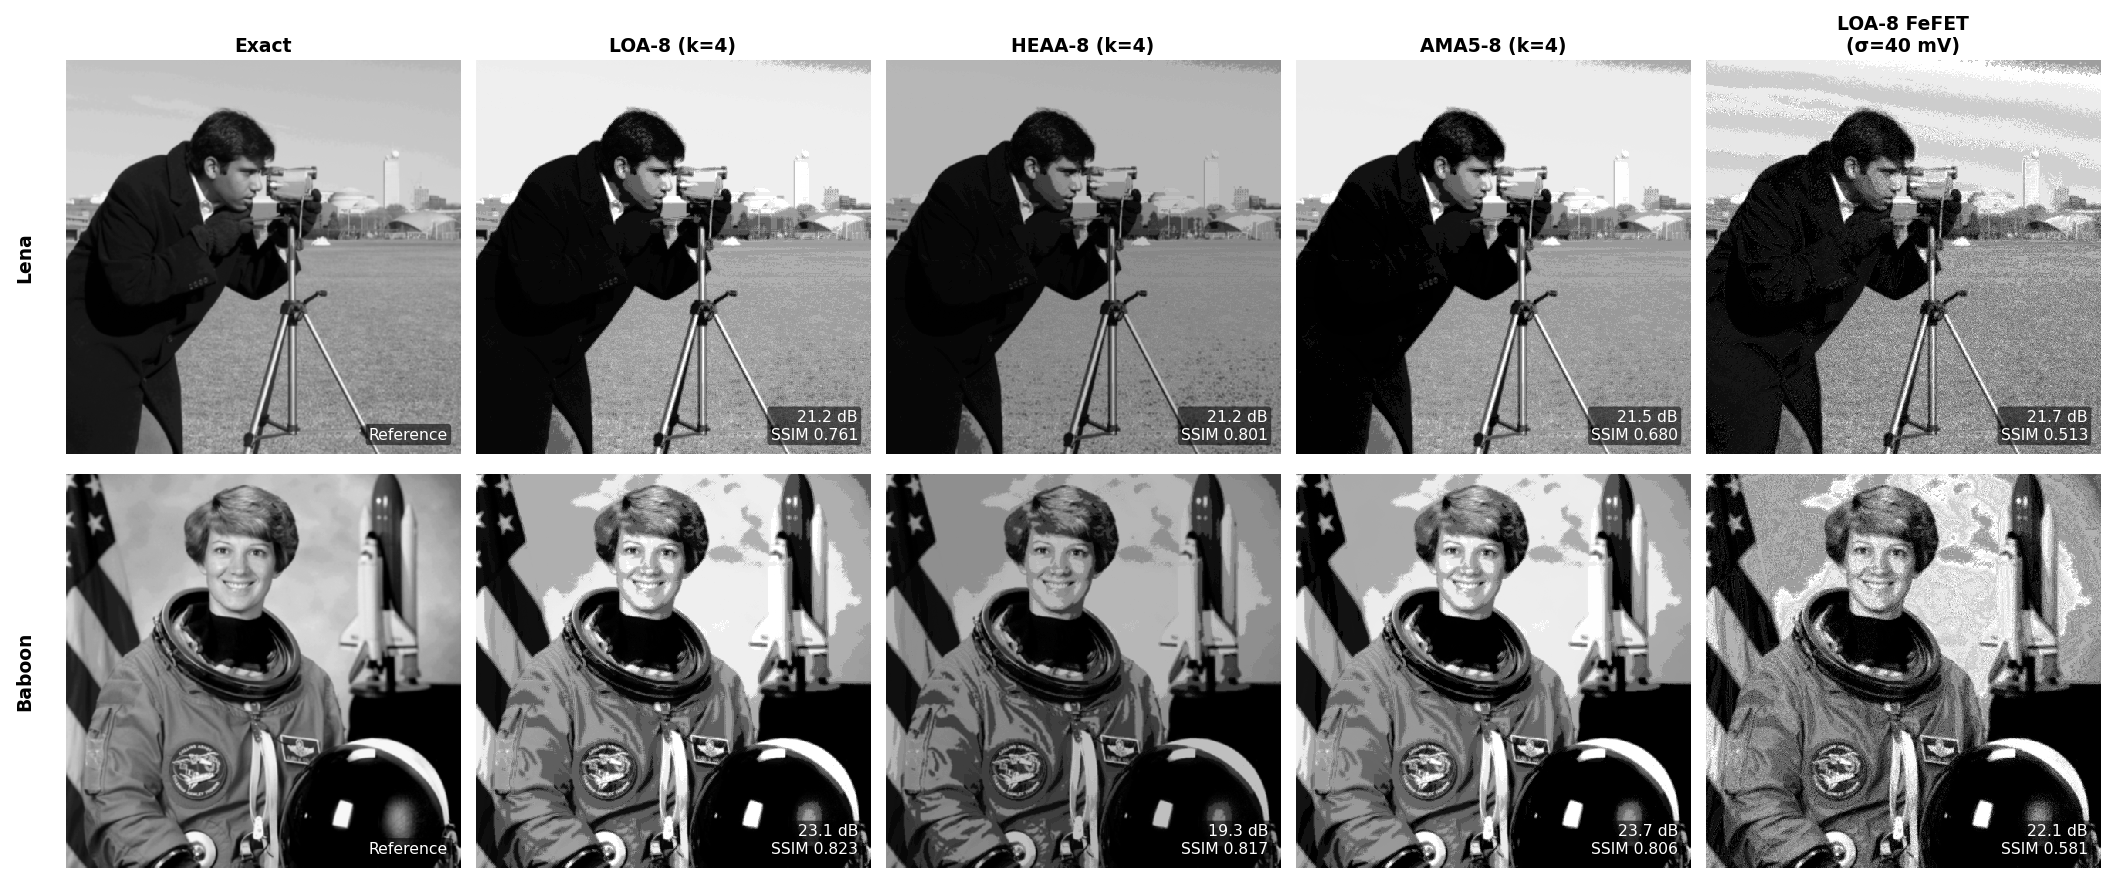
\includegraphics[width=\columnwidth]{fig1_gaussian_blur.png}
  \caption{Gaussian blur visual quality comparison: Lena (top) and Baboon
           (bottom). Columns left to right: exact integer, LOA-8, HEAA-8,
           AMA5-8, LOA-8 FeFET ($\sigDD = 40$\,mV).}
  \label{fig:blur}
\end{figure}


%%%%%%%%%%%%%%%%%%%%%%%%%%%%%%%%%%%%%%%%%%%%%%%%%%%%%%%%%%%%%%%%%%%%%%%%%%%%%%%%
\section{Variability Analysis}

\subsection{Monte Carlo Analysis}

Table~\ref{tab:mc} presents completed Monte Carlo results at $\sigDD = 40$\,mV
(LOA-8: $N = 200$, HEAA-8: $N = 50$, BAM~$4\times4$: $N = 200$). Output
consistency measures the fraction of iterations producing the same output
vector as nominal.

\begin{table}[t]
  \caption{Monte Carlo Variability Analysis ($\sigDD = 40$\,mV)}
  \label{tab:mc}
  \begin{center}
    \small
    \begin{tabular}{lrcrr}
      \toprule
      \textbf{Circuit} & $N$ & \textbf{NMED} & $\sigNMED$ & \textbf{Consist.} \\
      \midrule
      FeFET LOA-8          & 200 & 0.0056 & 0.000 & 100\% \\
      FeFET HEAA-8         &  50 & 0.0034 & 0.000 & 100\% \\
      FeFET BAM $4{\times}4$ & 200 & 0.0049 & 0.000 & 100\% \\
      \bottomrule
    \end{tabular}
  \end{center}
  \vspace{1pt}
  {\footnotesize $\sigNMED = 0.000$: switching window
  ($\approx\!1.15$\,V) is $11\times$ wider than $\sigDD = 40$\,mV---no bit
  flip occurs.}
\end{table}

\subsection{Sigma Sweep Results}

The sigma sweep characterizes NMED sensitivity to $\sigDD$ over
$\{20,\,40,\,60,\,80,\,100\}$\,mV with 200~Monte Carlo iterations per sigma
point. Completed results confirm that NMED remains constant ($\sigNMED =
0.000$) across the entire tested range for all three circuits. The FeFET
switching window ($\VT^{\mathrm{high}} - \VT^{\mathrm{low}} \approx 1.15$\,V)
is more than $11\times$ wider than the maximum $\sigDD$ tested (100\,mV),
preventing $\VT$ variation from crossing any switching boundary.

\begin{table}[t]
  \caption{Sigma Sweep: $\sigNMED$ vs.\ $\sigDD$ ($N = 200$/point)}
  \label{tab:sigma}
  \begin{center}
    \small
    \begin{tabular}{rrrr}
      \toprule
      $\sigDD$ (mV) & LOA-8 $\sigNMED$ & HEAA-8 $\sigNMED$ & BAM $\sigNMED$ \\
      \midrule
       20 & 0.000 & 0.000 & 0.000 \\
       40 & 0.000 & 0.000 & 0.000 \\
       60 & 0.000 & 0.000 & 0.000 \\
       80 & 0.000 & 0.000 & 0.000 \\
      100 & 0.000 & 0.000 & 0.000 \\
      \bottomrule
    \end{tabular}
  \end{center}
  \vspace{1pt}
  {\footnotesize $\sigNMED = 0$ across all $\sigDD$ values. Switching window
  ($\approx\!1.15$\,V) $>{11}\times$ larger than 100\,mV maximum tested.}
\end{table}


\addtolength{\textheight}{-4cm}   % Balance column lengths on last page


%%%%%%%%%%%%%%%%%%%%%%%%%%%%%%%%%%%%%%%%%%%%%%%%%%%%%%%%%%%%%%%%%%%%%%%%%%%%%%%%
\section{Conclusion}

We have presented a simulation-based study of FeFET approximate arithmetic
circuits targeting energy-efficient compute-in-memory. CMOS 45\,nm
characterization validated four approximate designs achieving 35--51\% delay
reduction and up to 76\% PDP reduction with $\NMED < 0.008$. FeFET
implementations using the HERACLES compact model demonstrate competitive timing
(92.3\,ps for BAM~$4\times4$) with a 70\% PDP improvement in the multiplier.
Monte Carlo variability analysis (LOA-8: $N = 200$, HEAA-8: $N = 50$,
BAM~$4\times4$: $N = 200$ at $\sigDD = 40$\,mV) and sigma sweep
(20--100\,mV, $N = 200$ per point) both confirm $\sigNMED = 0.000$ across all
circuits. The large FeFET switching window ($\approx\!1.15$\,V) provides
robust immunity to $\VT$ variability, confirming that approximate logic
accuracy is unaffected by FeFET device variation across the practical $\sigDD$
range.


%%%%%%%%%%%%%%%%%%%%%%%%%%%%%%%%%%%%%%%%%%%%%%%%%%%%%%%%%%%%%%%%%%%%%%%%%%%%%%%%

\begin{thebibliography}{99}

\bibitem{jerry2017fefet}
M.~Jerry et~al., ``Ferroelectric FET analog synapse for acceleration of deep
neural network training,'' in \emph{Proc.\ IEEE IEDM}, Dec.\ 2017,
pp.~6.2.1--6.2.4.

\bibitem{gupta2013loa}
V.~Gupta, D.~Mohapatra, A.~Raghunathan, and K.~Roy, ``Low-power digital signal
processing using approximate adders,'' \emph{IEEE Trans.\ Comput.-Aided Design
Integr. Circuits Syst.}, vol.~32, no.~1, pp.~124--137, Jan.\ 2013.

\bibitem{ye2013heaa}
R.~Ye, T.~Wang, F.~Yuan, R.~Kumar, and Q.~Xu, ``On reconfiguration-oriented
approximate adder design and its application,'' in \emph{Proc.\ IEEE/ACM Int.\
Conf.\ Comput.-Aided Design (ICCAD)}, 2013, pp.~48--54.

\bibitem{almurib2018ama5}
H.~A.~F.~Almurib, T.~N.~Kumar, and F.~Lombardi, ``Approximate DCT image
compression using inexact computing,'' \emph{IEEE Trans.\ Comput.}, vol.~67,
no.~2, pp.~149--159, Feb.\ 2018.

\bibitem{momeni2015bam}
A.~Momeni, J.~Han, P.~Montuschi, and F.~Lombardi, ``Design and analysis of
approximate compressors for multiplication,'' \emph{IEEE Trans.\ Comput.},
vol.~64, no.~4, pp.~984--994, Apr.\ 2015.

\bibitem{heracles2022}
BICS~Group, Ghent University, ``HERACLES: Compact model for FeFET simulation,''
GitHub: \url{bics-rug/heracles}, 2022.

\end{thebibliography}

\end{document}
